\section{Experimentos e Resultados}

Para comparar o desempenho das arquiteturas propostas, realizamos o benchmark YCSB com as configurações do Cassandra descritas na Seção de Sistema Proposto.
Os resultados estão descritos a seguir, com foco em throughput, latência e overheads de cada configuração.

\subsection{Resultados do Benchmark YCSB}
\begin{table}[H]
\centering
\caption{Tempos de benchmark no YCSB}
\begin{tabular}{lcc}
\hline
Configuração & Tempo de Carregamento (ms) & Tempo de Execução (ms) \\
\hline
Nó único & 386\,275 & 625\,923 \\
3 nós sem replicação  & 224\,126 & 225\,164 \\
3 nós com replicação  & 477\,892 & 552\,229 \\
\hline
\end{tabular}
\end{table}

\begin{table}[H]
    \centering
	\small
    \caption{Resultados do benchmark YCSB - Único nó}
    \begin{tabular}{lcccccc}
    \hline
	Operação & Operações & Latência Média (\textmu s) & Latência Mín (\textmu s) & Latência Máx (\textmu s) & 95\% (\textmu s) & 99\% (\textmu s) \\
	\hline
	INSERT   & 10\,000\,000 & 1\,222,82 & 197   & 148\,607 & 1\,961 & 5\,299 \\
	READ     & 5\,000\,753  & 2\,296,55 & 220   & 135\,295 & 4\,583 & 11\,775 \\
	UPDATE   & 4\,999\,247  & 1\,681,11 & 159   & 149\,759 & 2\,923 & 7\,011 \\
	\hline
    \end{tabular}
    \end{table}

    \begin{table}[H]
    \centering
	\small
    \caption{Resultados agregados do benchmark YCSB - 3 nós sem replicação}
    \begin{tabular}{lrrrrrr}
    \hline
	Operação & Operações & Latência Média (\textmu s) & Latência Mín (\textmu s) & Latência Máx (\textmu s) & 95\% (\textmu s) & 99\% (\textmu s) \\
	\hline
	INSERT   & 10\,000\,000 & 703,01 & 159 & 139\,135 & 1\,084 & 2\,669 \\
	READ     & 4\,998\,961  & 759,82 & 210 & 97\,151  & 1\,205 & 2\,307 \\
	UPDATE   & 5\,001\,039  & 656,09 & 160 & 95\,935  & 1\,087 & 1\,964 \\
	\hline
    \end{tabular}
    \end{table}

    \begin{table}[H]
    \centering
	\small
    \caption{Resultados agregados do benchmark YCSB - 3 nós com replicação} 
    \begin{tabular}{lrrrrrr}
    \hline
	Operação & Operações & Latência Média (\textmu s) & Latência Mín (\textmu s) & Latência Máx (\textmu s) & 95\% (\textmu s) & 99\% (\textmu s) \\
	\hline
	INSERT   & 10\,000\,000 & 1\,514,36 & 186 & 149\,119 & 3\,843 & 9\,103 \\
	READ     & 5\,000\,119  & 2\,334,83 & 268 & 125\,119 & 5\,563 & 11\,191 \\
	UPDATE   & 4\,999\,881  & 1\,170,27 & 182 & 114\,431 & 3\,099 & 5\,983 \\
	\hline
    \end{tabular}
    \end{table}

\subsection{Análise Comparativa dos Resultados}

A análise dos resultados obtidos evidencia diferenças significativas no desempenho das configurações avaliadas.
O cluster com três nós sem replicação apresentou as menores latências médias para todas as operações (INSERT, READ e UPDATE),
demonstrando maior eficiência na distribuição da carga e no processamento das requisições.

A configuração com replicação no cluster de três nós resultou em um aumento considerável nas médias das latências,
especialmente nas operações de escrita e leitura. 
Esse aumento pode ser atribuído ao overhead inerente ao mecanismo de replicação, que demanda sincronização adicional entre os nós do cluster.

Comparando-se o desempenho do nó único com as demais configurações,
observa-se que  apresentou métricas semelhantes em relação à configuração de cluster com replicação, entretanto não dispõe dos mesmos níveis de disponibilidade e tolerância a falhas.

\subsubsection{Análise dos Recursos Utilizados no Cluster}
Além das métricas de latência e throughput, decidimos comparar o uso de recursos do cluster durante a execução do benchmark YCSB.
Abaixo estão os gráficos de uso de recursos dos nós que compõem cada cluster:
\begin{figure}[H]
	\captionsetup{labelformat=empty}
  	\caption{Sem Replicação}
	\centering
  \begin{minipage}{0.32\linewidth}
    \centering
    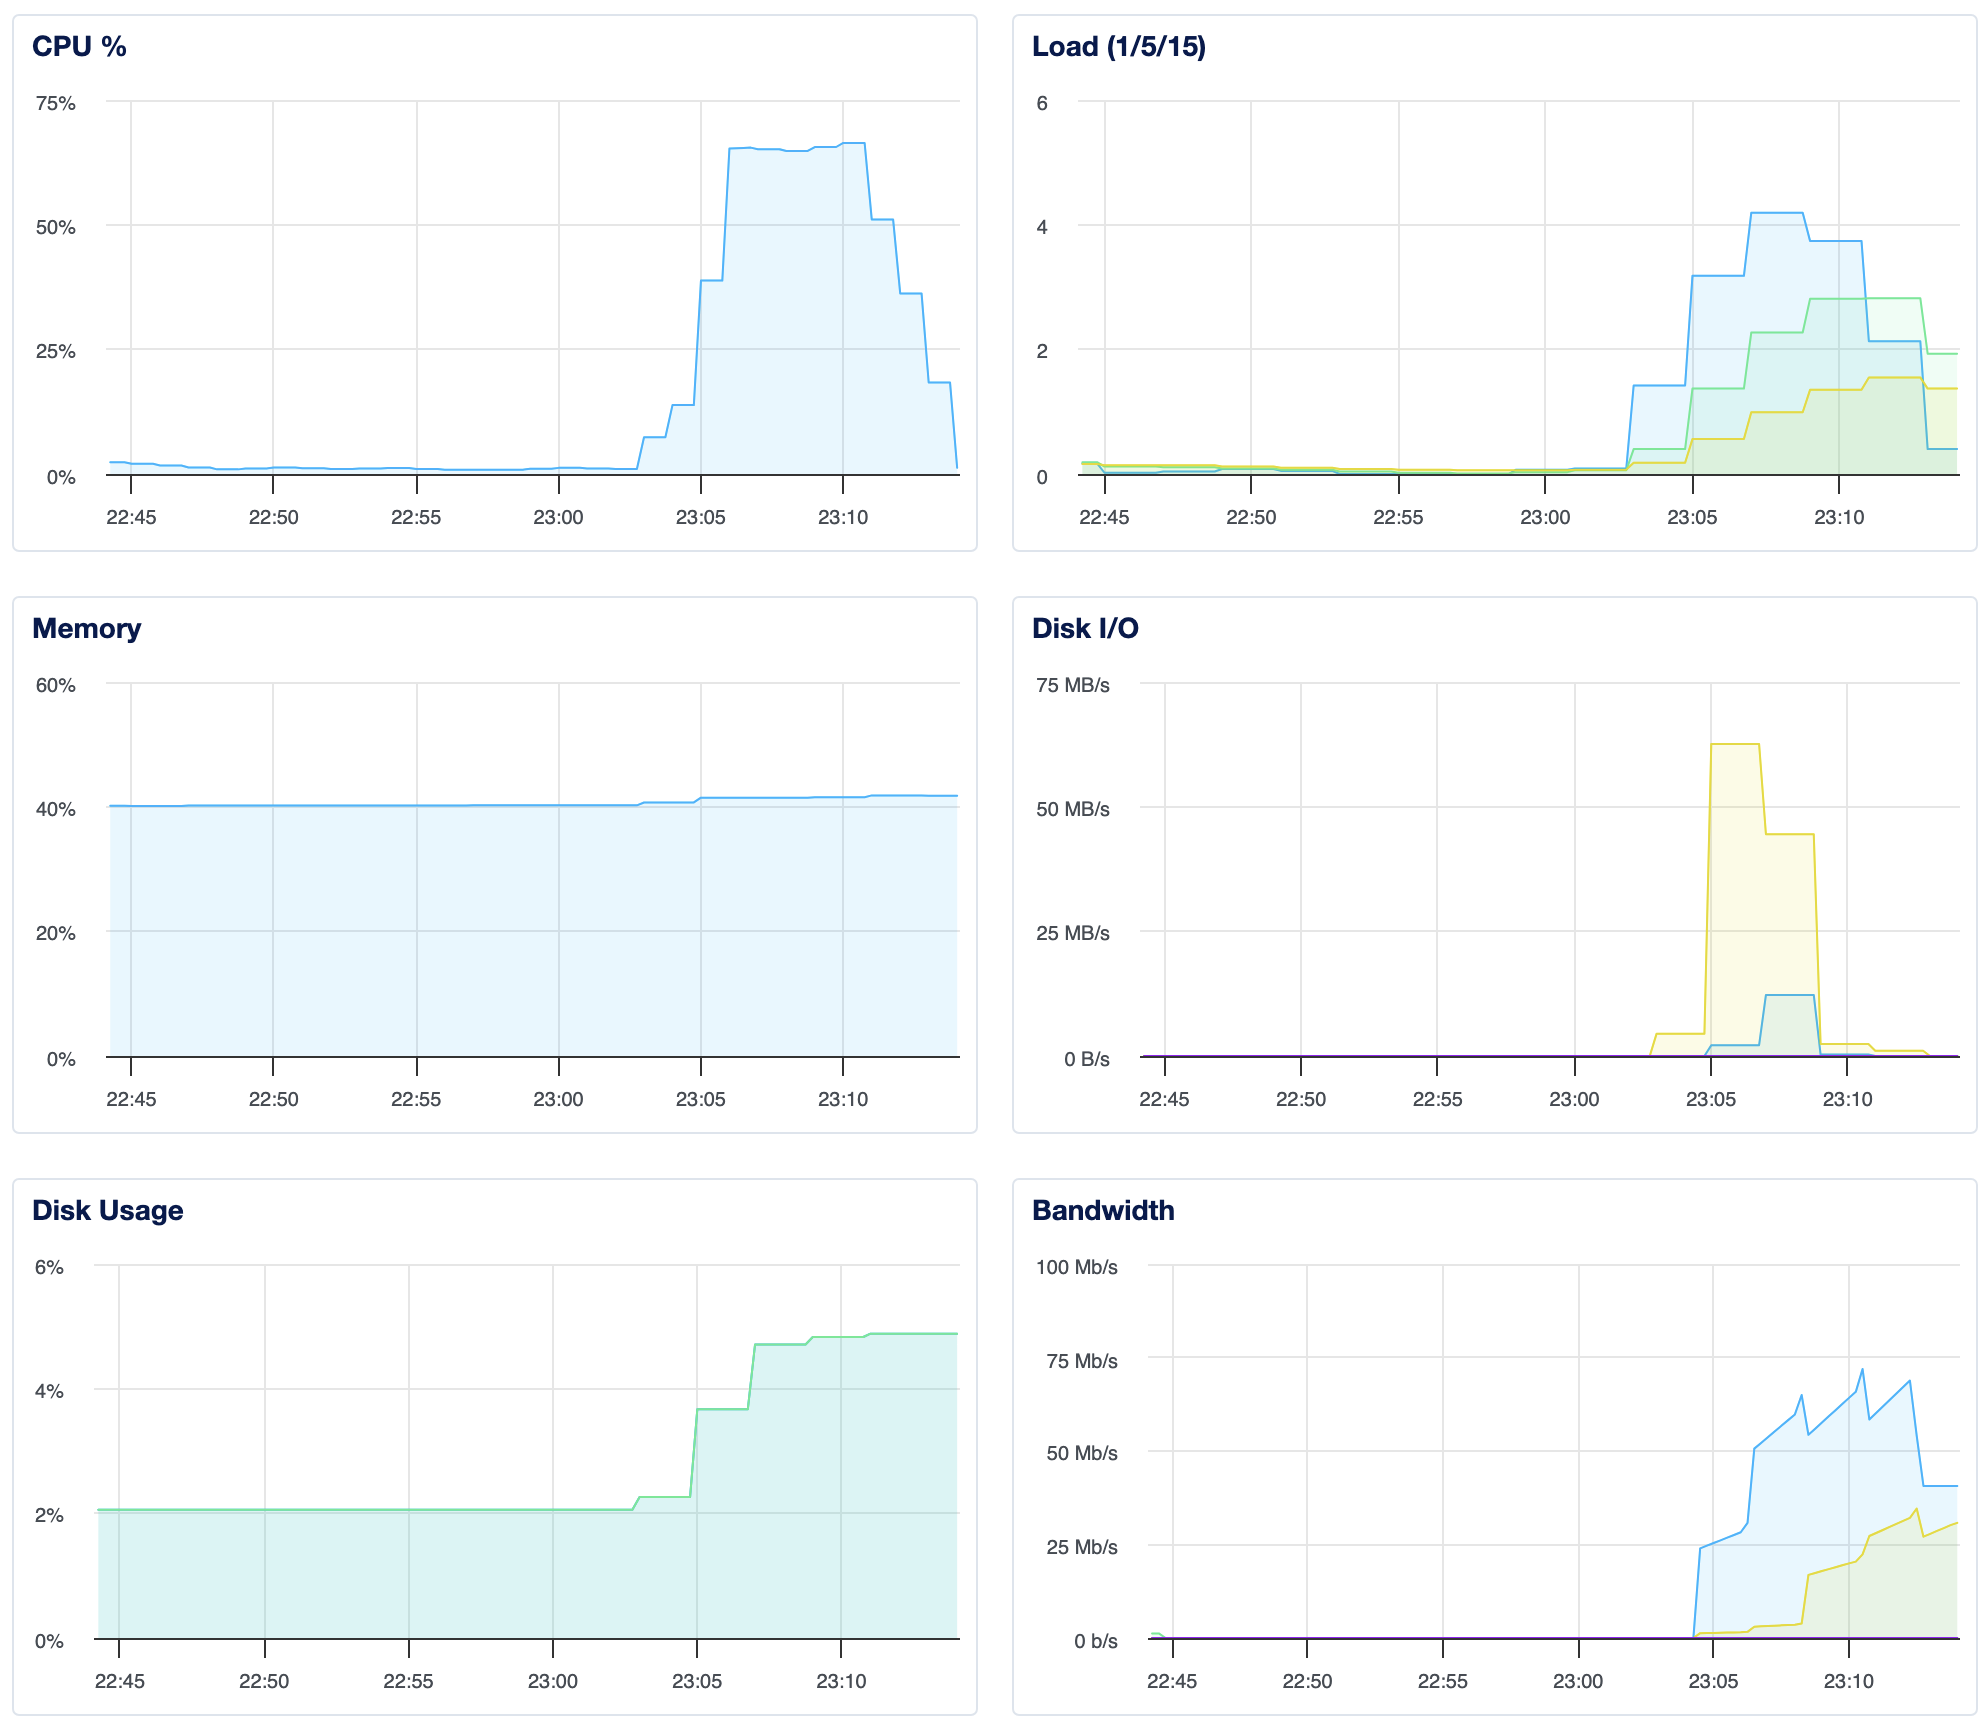
\includegraphics[width=\linewidth]{imgs/3-1-01.png}
    \caption{Nó 1}
  \end{minipage}
  \hfill
  \begin{minipage}{0.32\linewidth}
    \centering
    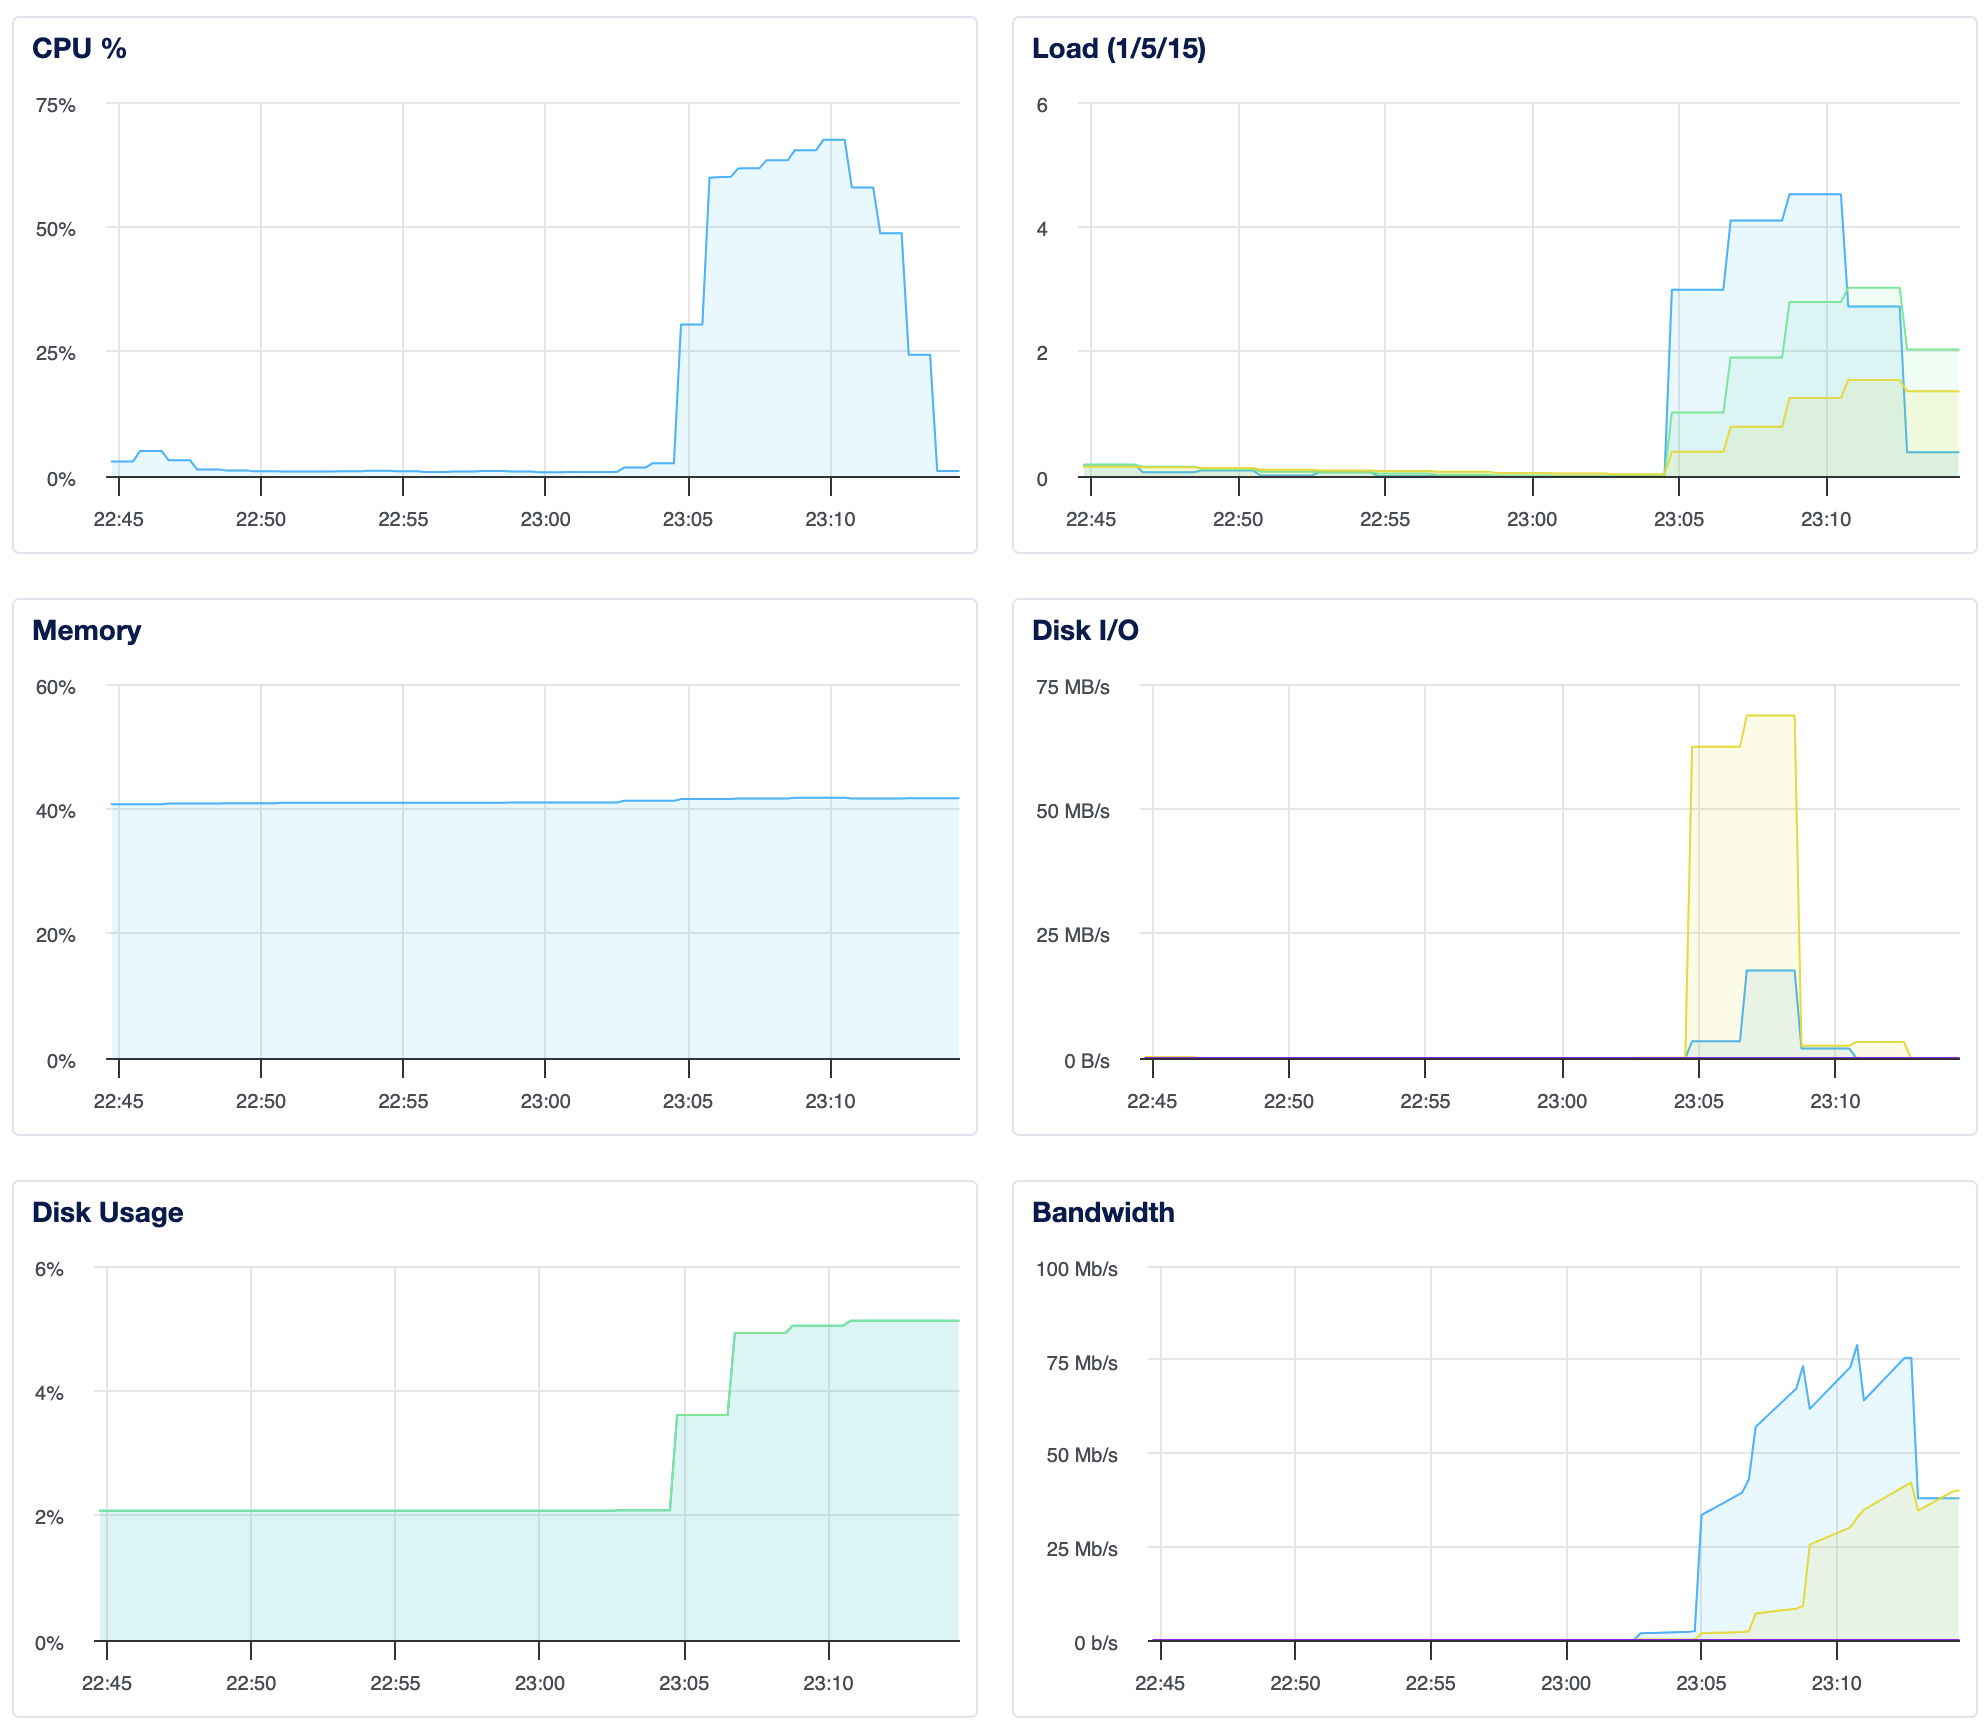
\includegraphics[width=\linewidth]{imgs/3-1-02.png}
    \caption{Nó 2}
  \end{minipage}
  \hfill
  \begin{minipage}{0.32\linewidth}
    \centering
    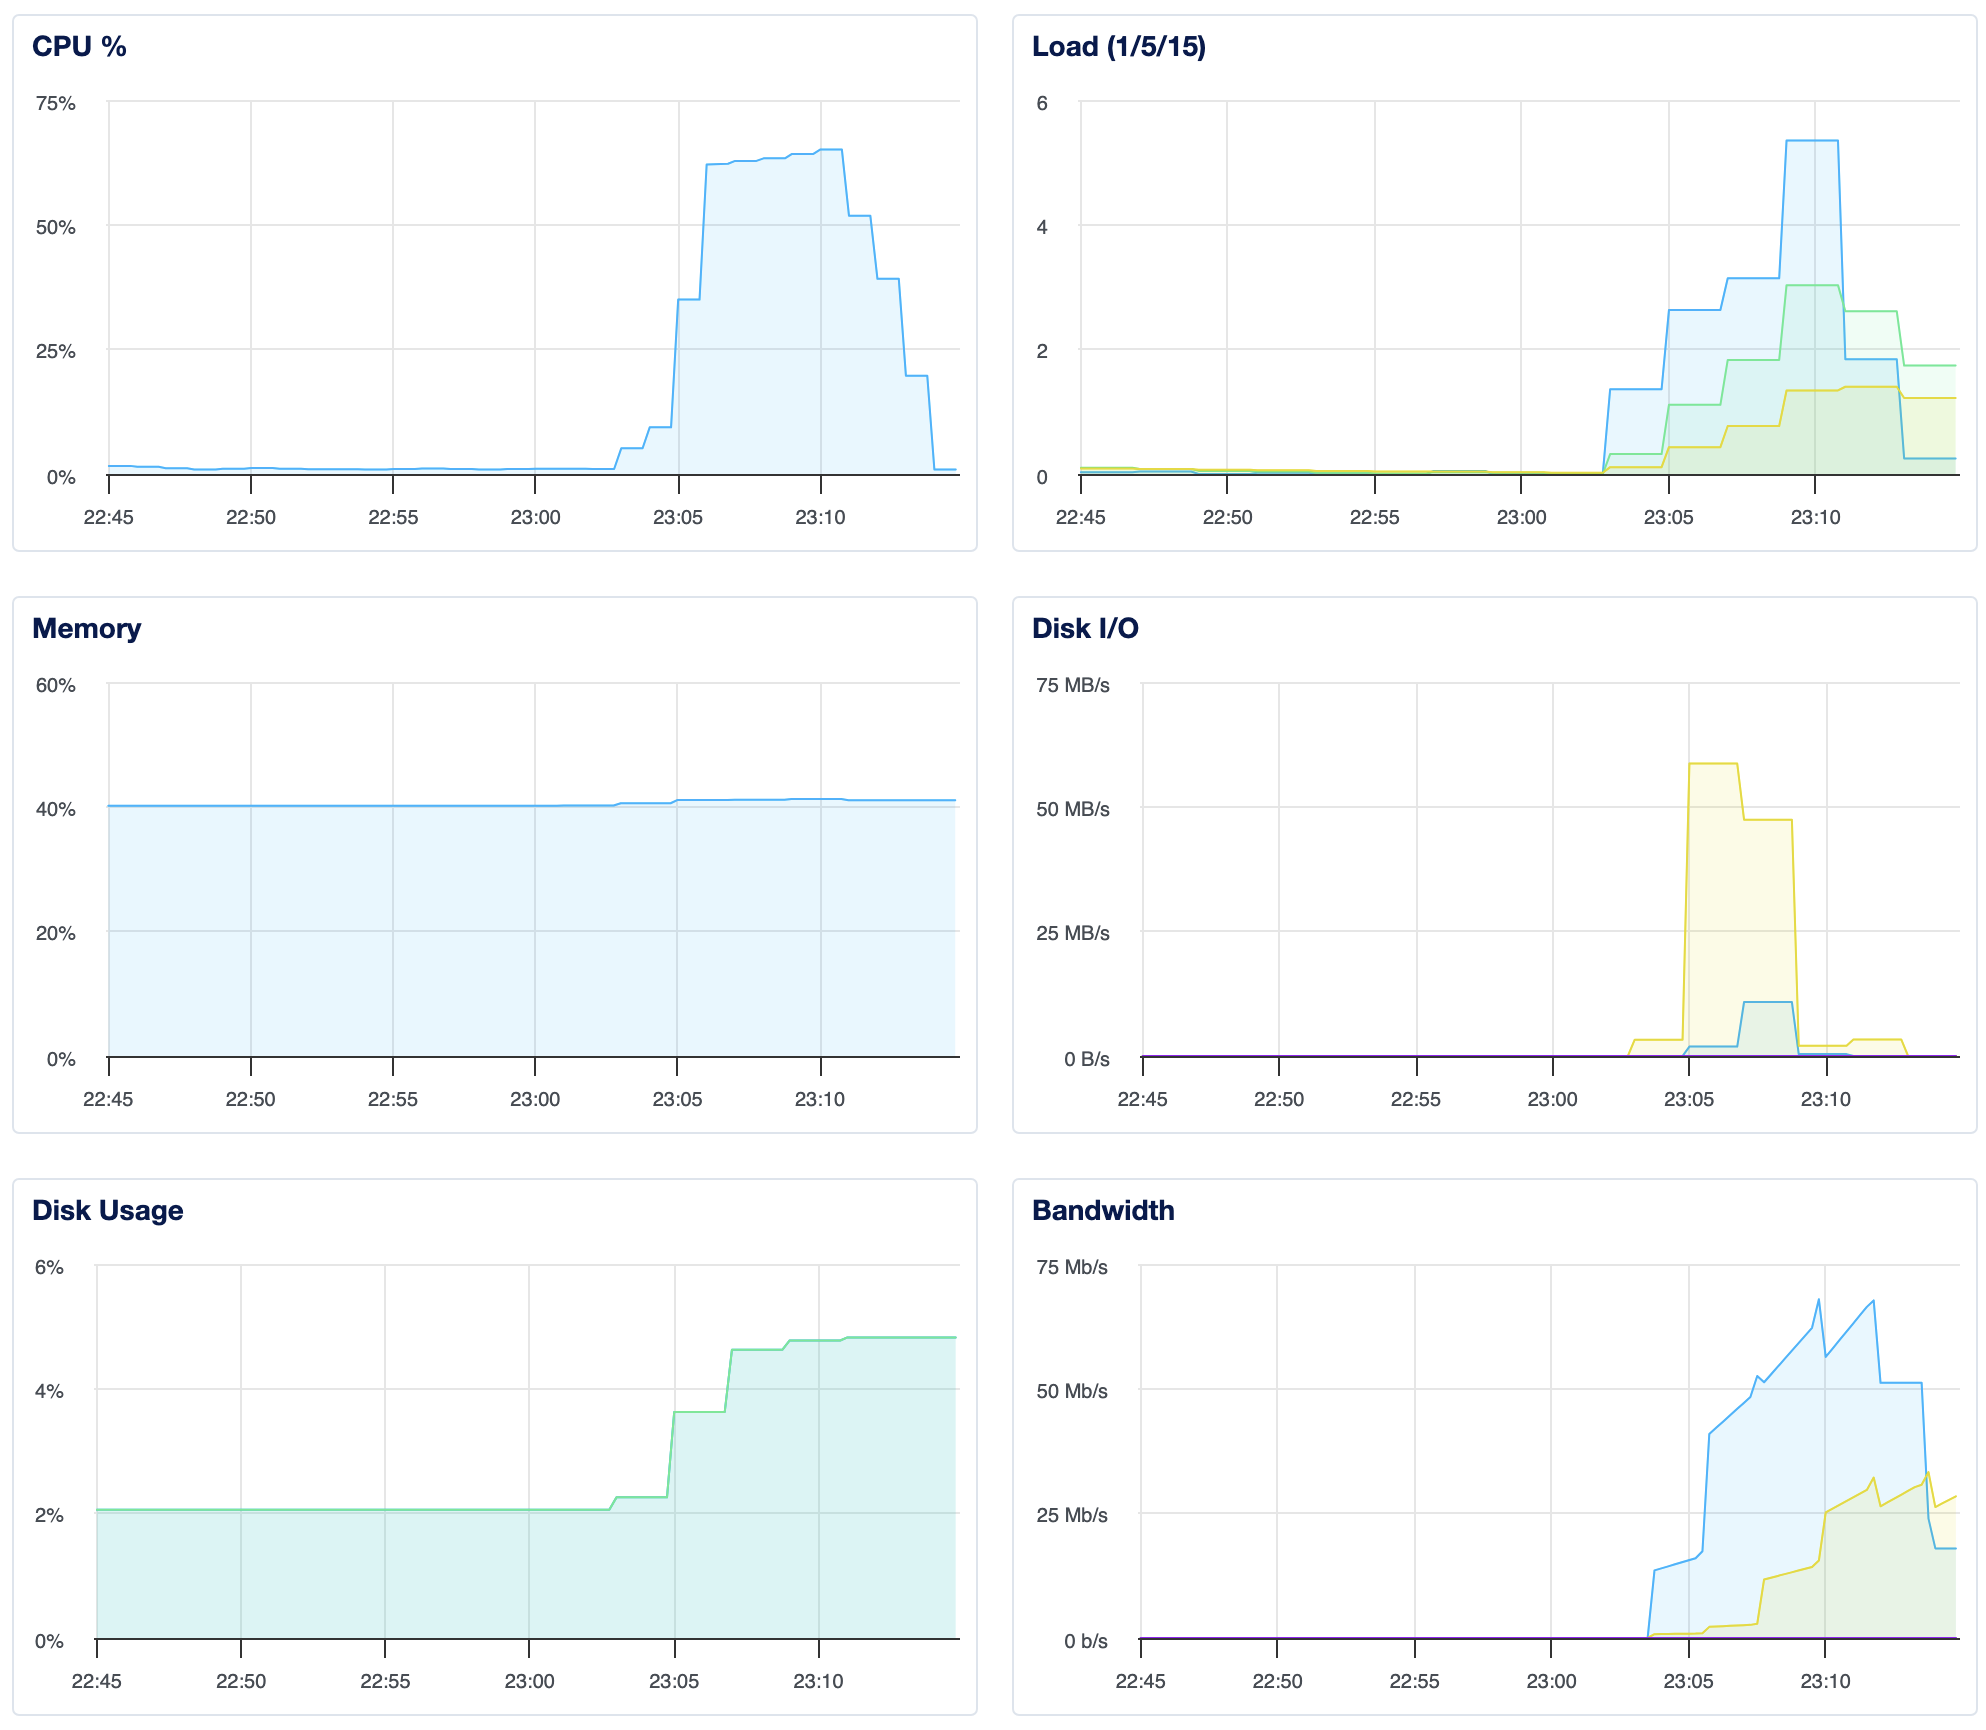
\includegraphics[width=\linewidth]{imgs/3-1-03.png}
    \caption{Nó 3}
  \end{minipage}
\end{figure}

\begin{figure}[H]
	\captionsetup{labelformat=empty}
	\caption{Com Replicação}
  \centering
  \begin{minipage}{0.32\linewidth}
    \centering
    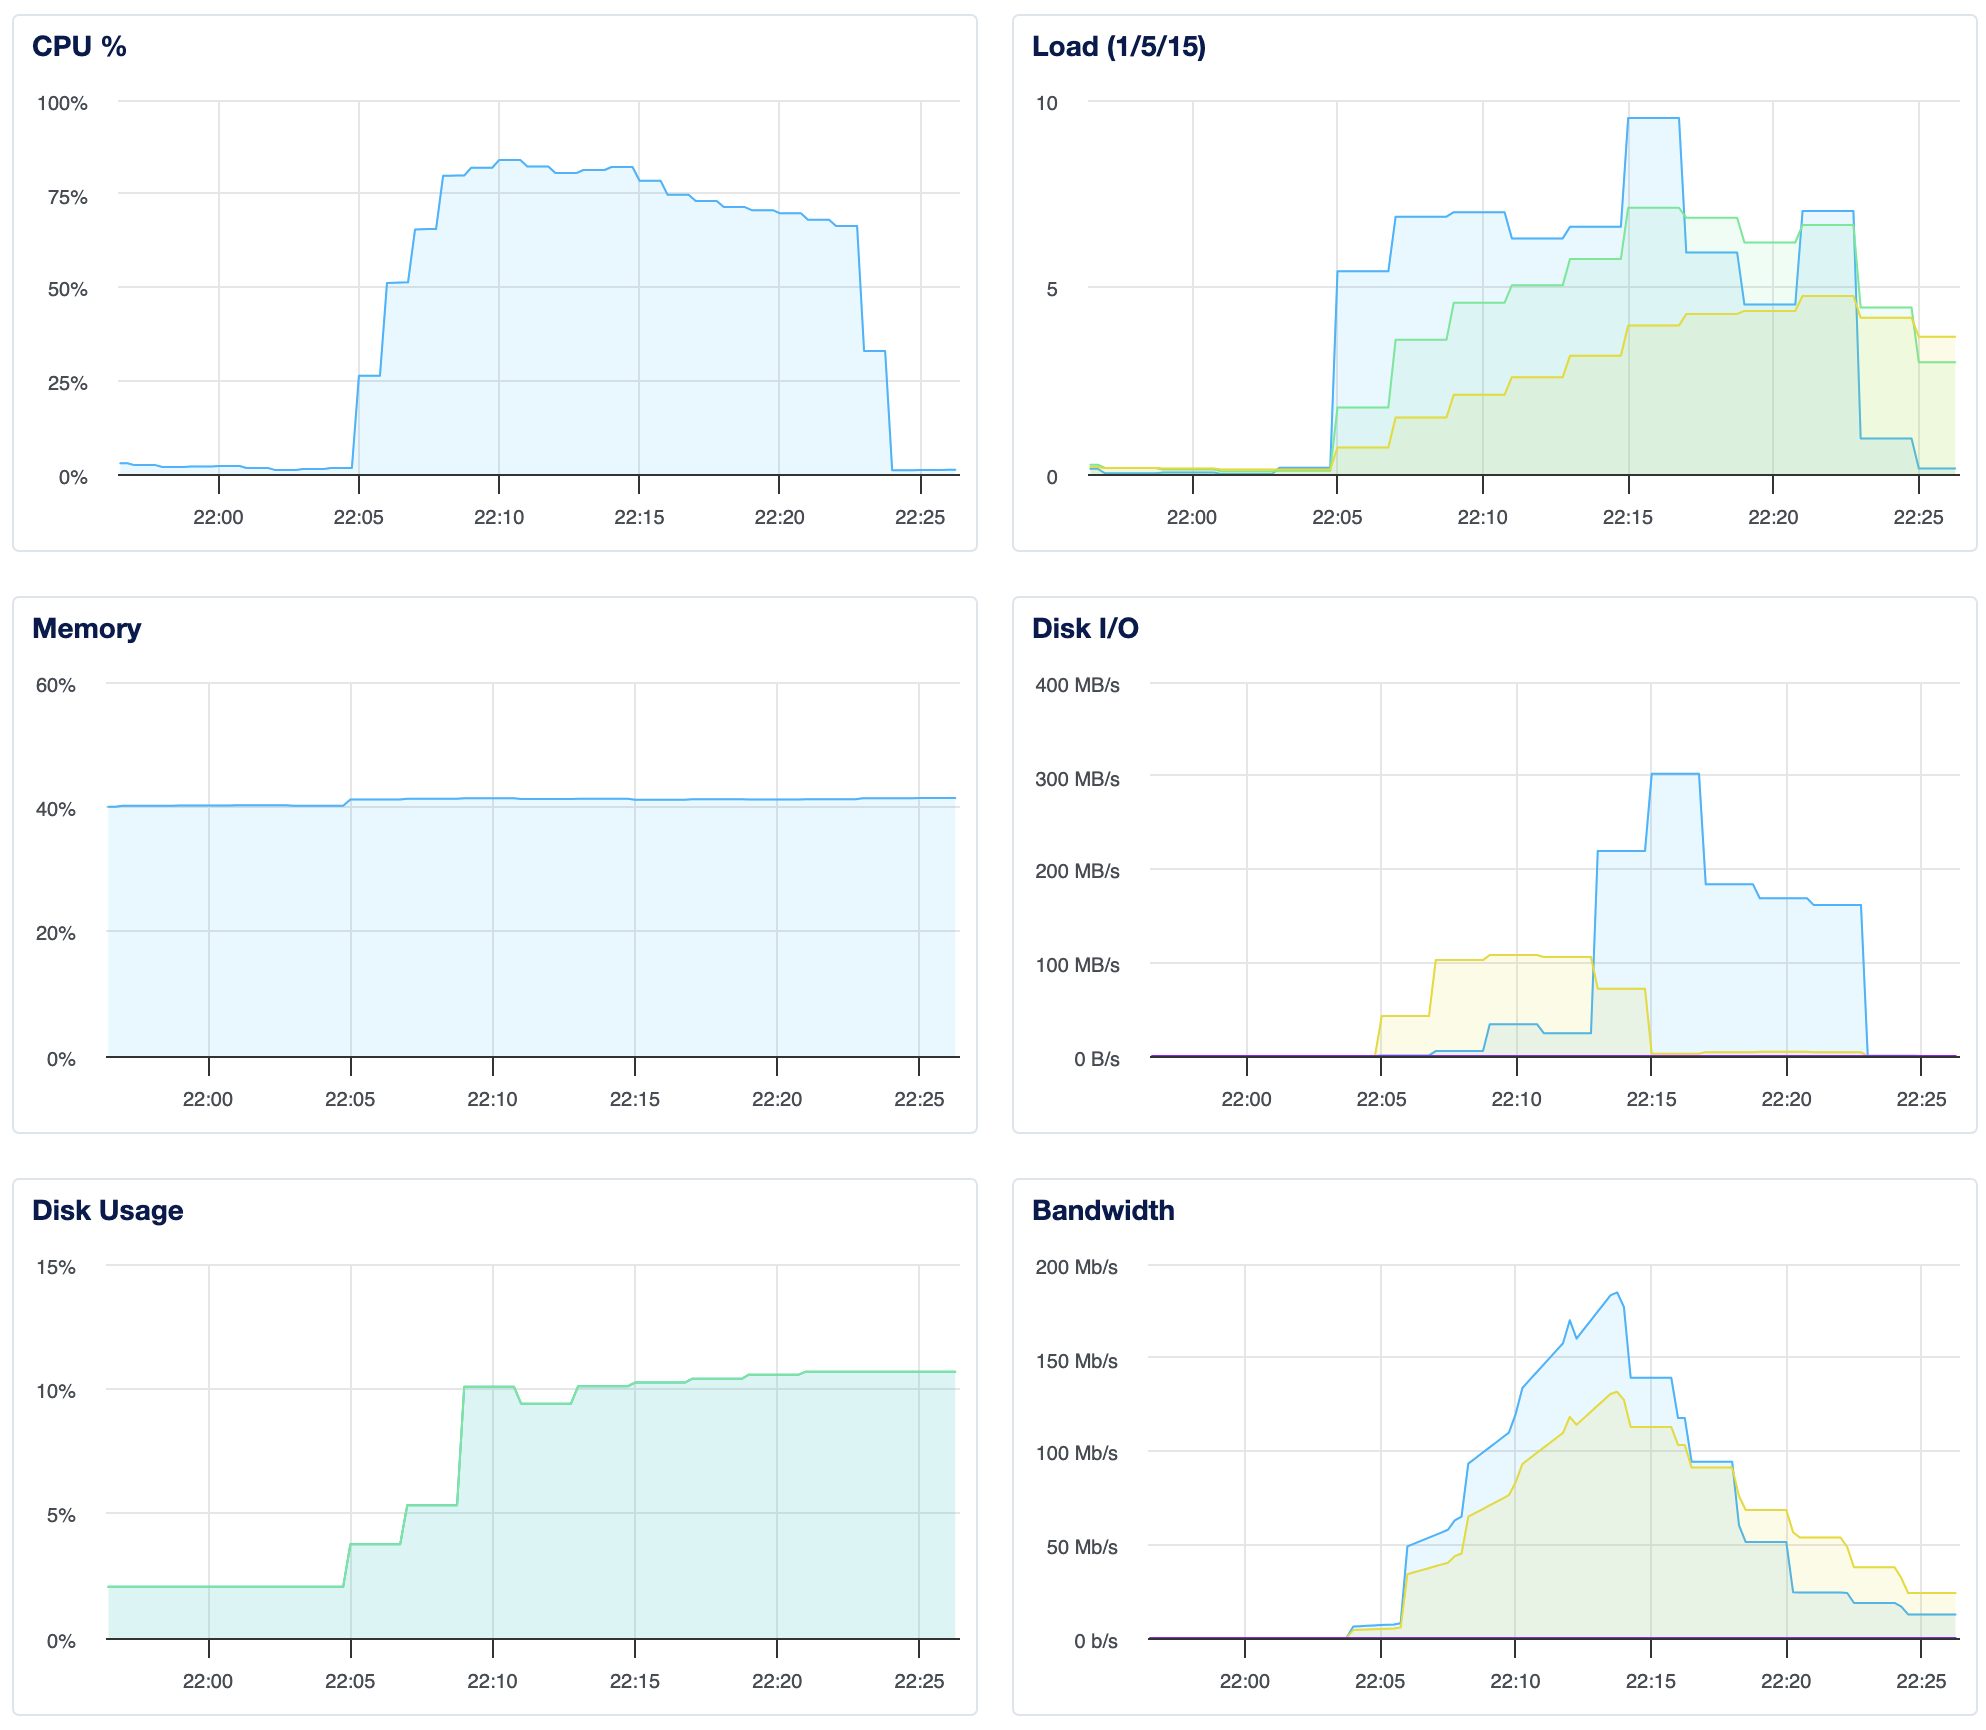
\includegraphics[width=\linewidth]{imgs/3-3-01.png}
    \caption{Nó 1}
  \end{minipage}
  \hfill
  \begin{minipage}{0.32\linewidth}
    \centering
    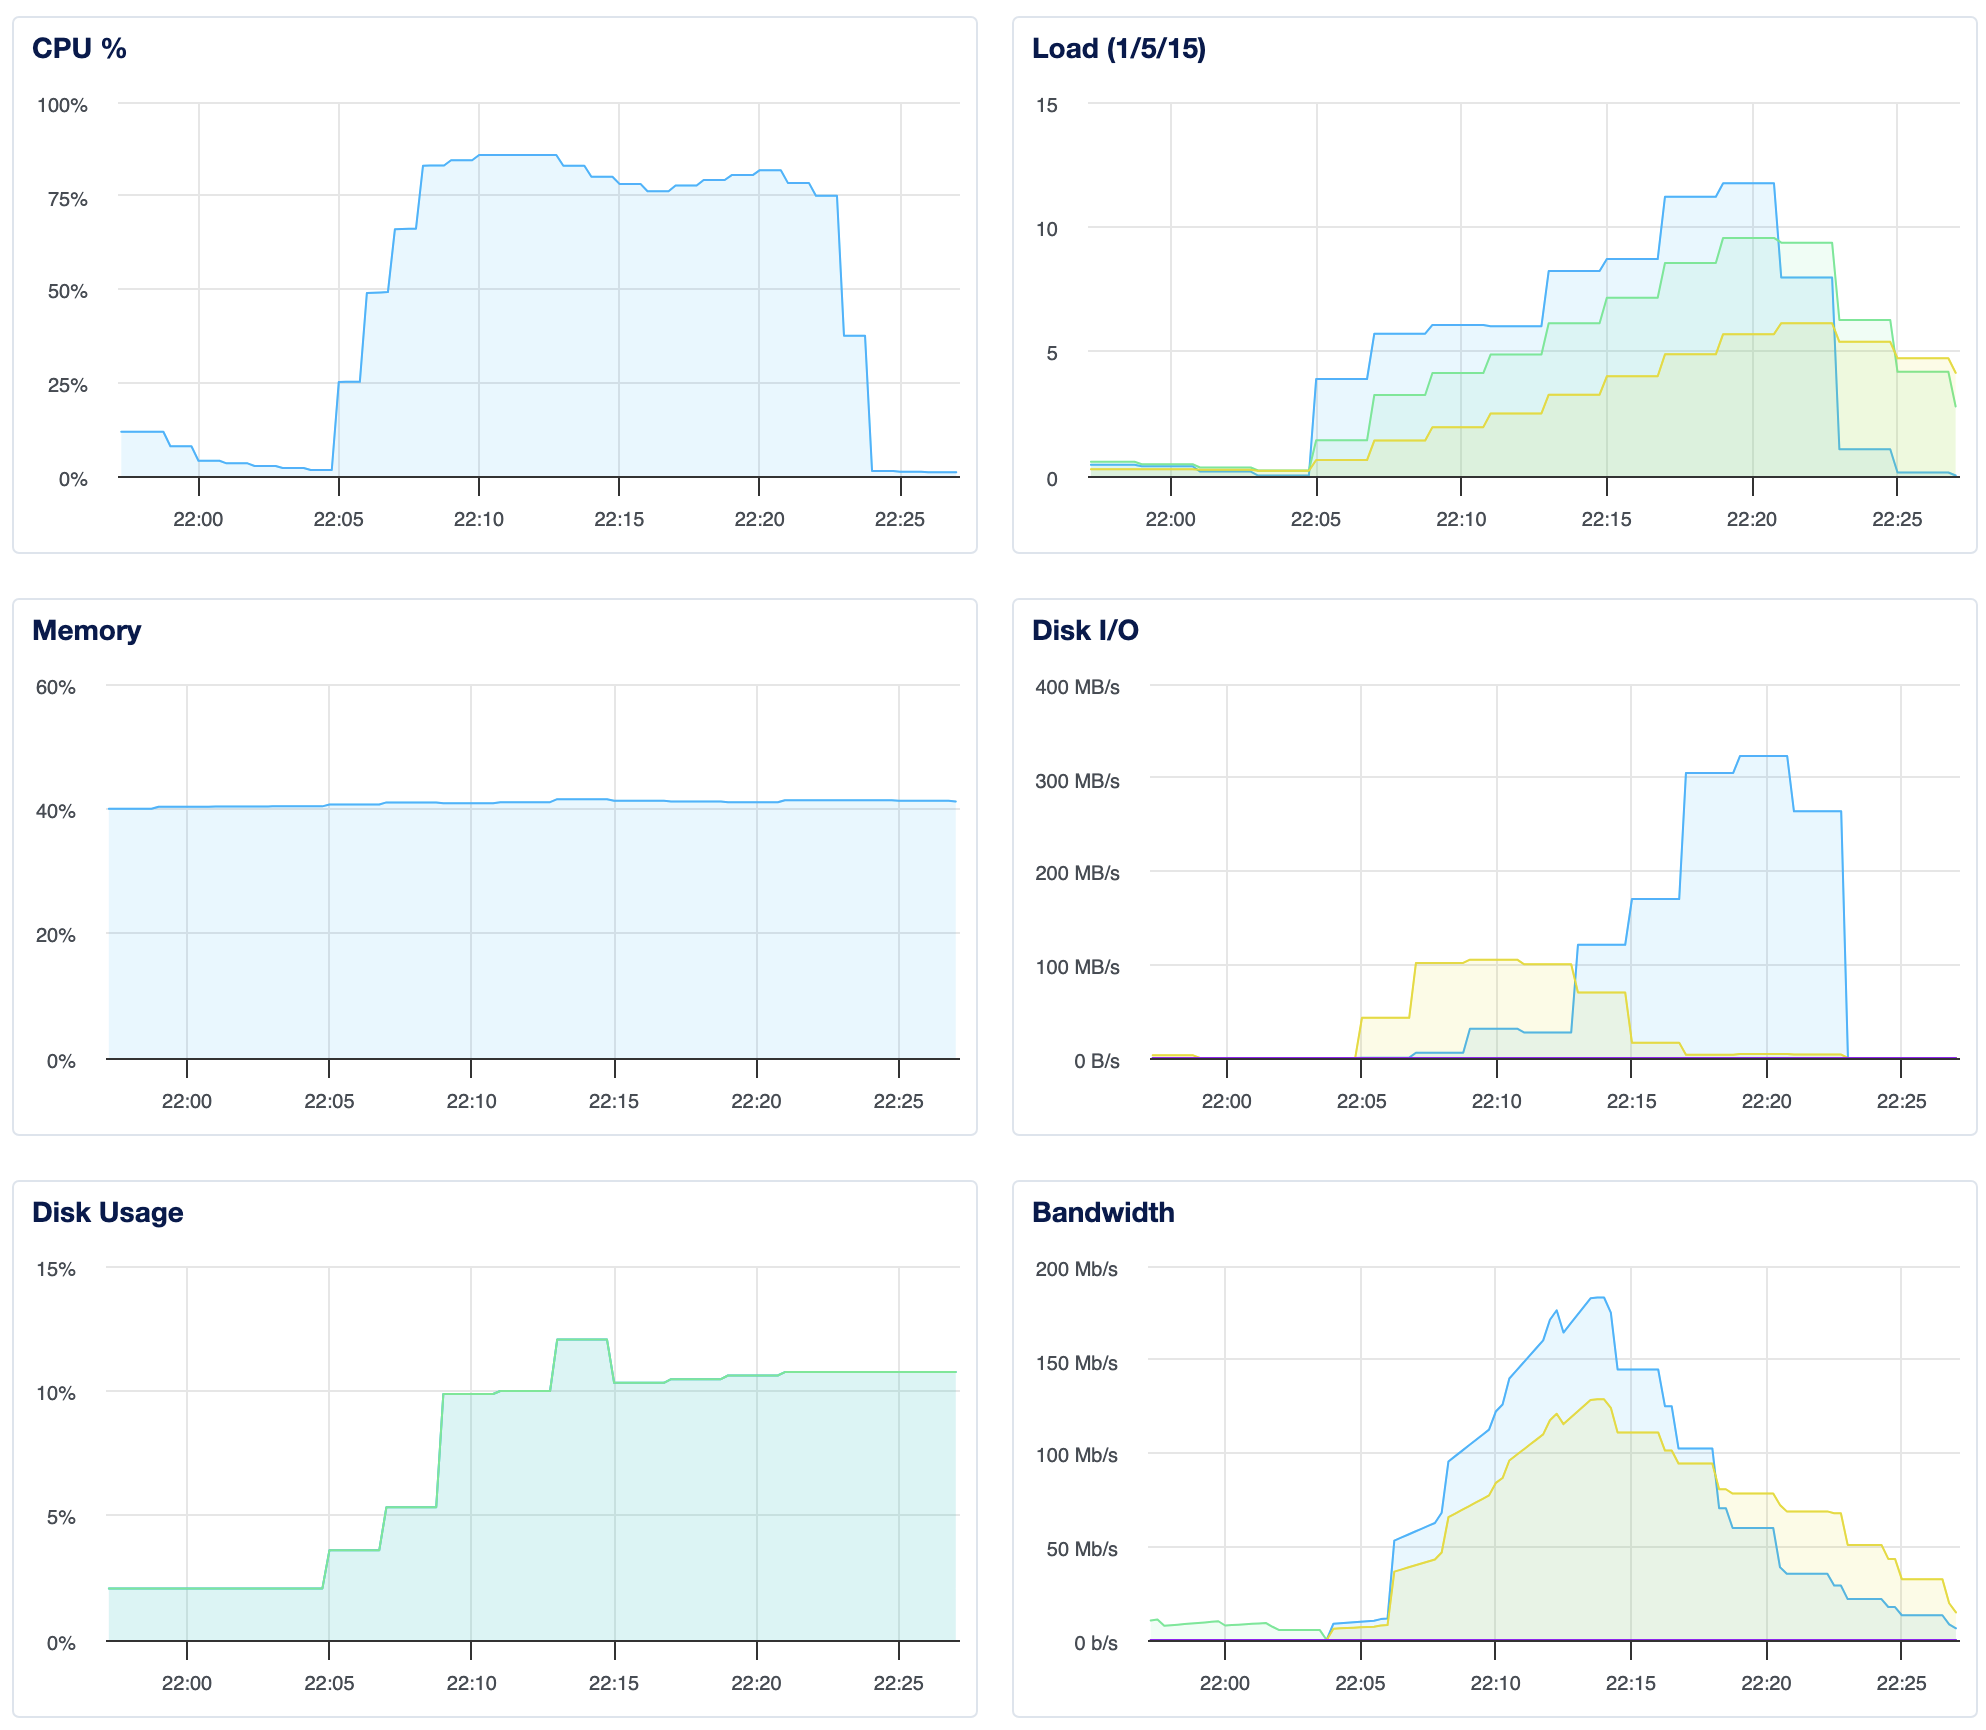
\includegraphics[width=\linewidth]{imgs/3-3-02.png}
    \caption{Nó 2}
  \end{minipage}
  \hfill
  \begin{minipage}{0.32\linewidth}
    \centering
    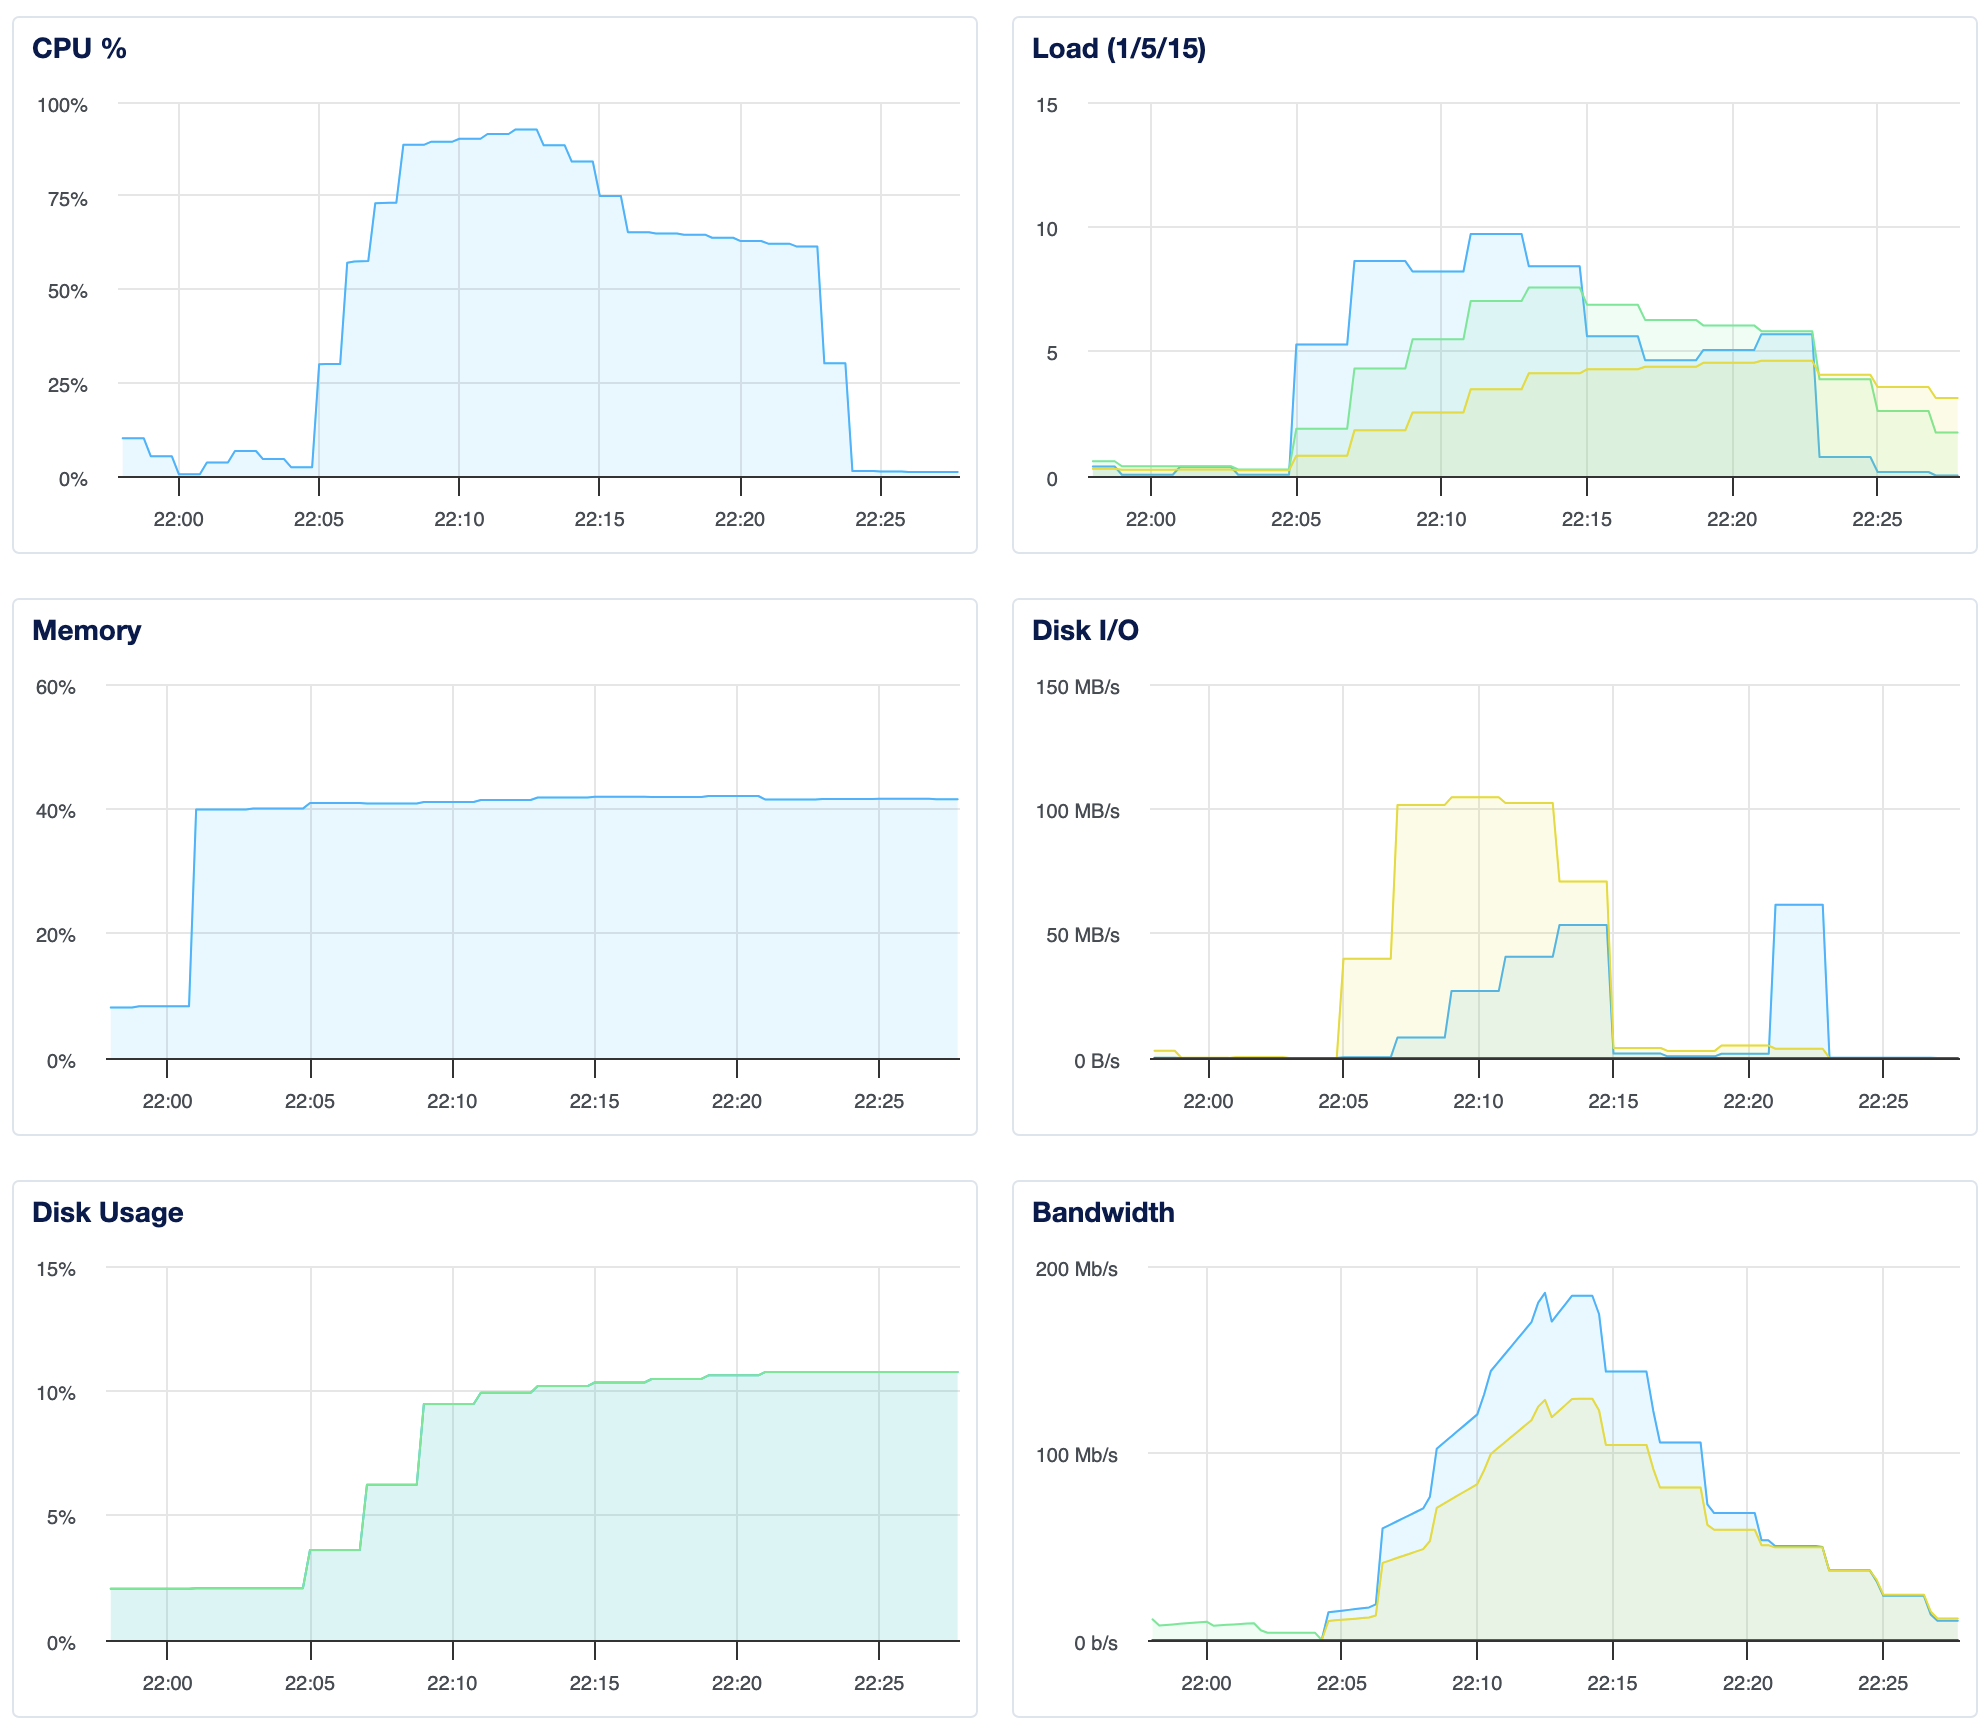
\includegraphics[width=\linewidth]{imgs/3-3-03.png}
    \caption{Nó 3}
  \end{minipage}
\end{figure}

Comparando o gráfico do uso de recursos do cluster sem replicação com o do cluster com replicação, observamos que para as arquiteturas utilizadas,
com excessão do uso de memória semelhante, todas métricas apresentam um aumento significativo no uso de recursos quando a replicação é ativada.
As métricas de leitura e escrita de disco e de uso de rede são as que mais se destacam, sendo que os clusters com replicação superaram em mais do dobro do uso desses recursos pelos cluster sem replicação.

De modo geral, obsevarmos que o overhead causado pela replicação é significativo, tanto em tempo como uso de recursos, 
mas é um custo necessário em aplicações que exijam maior disponibilidade e tolerância a falhas.
Para ambientes em que a latência é o principal critério de desempenho, a configuração de cluster sem replicação se mostra mais adequada.
